\documentclass[11pt]{article}
\usepackage[margin=1in]{geometry}
\usepackage[T1]{fontenc}
\usepackage{lmodern}
\usepackage{graphicx}
\usepackage{tikz}
\usepackage{float}
\usepackage{array}
\usepackage{setspace}
\usepackage[hidelinks]{hyperref}

\renewcommand{\arraystretch}{1.15}
\setlength{\parskip}{0.4em}
\setlength{\parindent}{0pt}
\onehalfspacing

\title{\textbf{Design Document}\\[0.5em]\large CNN Accelerator on DE1-SoC}
\author{Haoyu Lu}
\date{April 2026}

\begin{document}

\begin{titlepage}
\centering
\vspace*{3cm}
{\LARGE \textbf{Design Document}\par}
\vspace{0.8cm}
{\Large CNN Accelerator on DE1-SoC\par}
\vspace{2cm}
{\large Haoyu Lu\par}
\vspace{0.5cm}
{\large April 2026\par}
\vfill
\end{titlepage}

\tableofcontents
\newpage

\section{Introduction}

This project implements a CNN inference accelerator on Intel's DE1-SoC
platform. The design keeps the original accelerator datapath in FPGA logic and
adds a memory-mapped wrapper so that the HPS can load model parameters, provide
input images, trigger inference, and read back the predicted class. The overall
goal is to preserve the existing RTL structure while making the accelerator
usable from Linux software running on the ARM cores.

At a high level, the design is split into three layers:
\begin{itemize}
\item a CNN datapath in the FPGA fabric, rooted at \texttt{system\_top}
\item an MMIO wrapper, \texttt{cnn\_mmio\_interface}, that converts HPS register
and scratchpad accesses into the existing 32-bit streaming load interface
\item HPS-side software that uses \texttt{/dev/mem} to access the peripheral and
execute model-load and inference transactions
\end{itemize}

\section{System Block Diagram}

Figure~\ref{fig:system-block-diagram} shows the overall organization of the
project. Software runs on the HPS under Linux and accesses the FPGA peripheral
through the HPS-to-FPGA lightweight bridge. The MMIO wrapper provides a 16-bit
register space and a 16-bit scratchpad memory. It stages model data and input
samples, then replays them into the original \texttt{system\_top} load stream.
Inside \texttt{system\_top}, control is handled by \texttt{TopFSM} and
\texttt{LayerRunnerFSM}, while the computation is performed by the
convolution/quantization/pooling pipeline and the final fully-connected stage.

\begin{figure}[H]
\centering
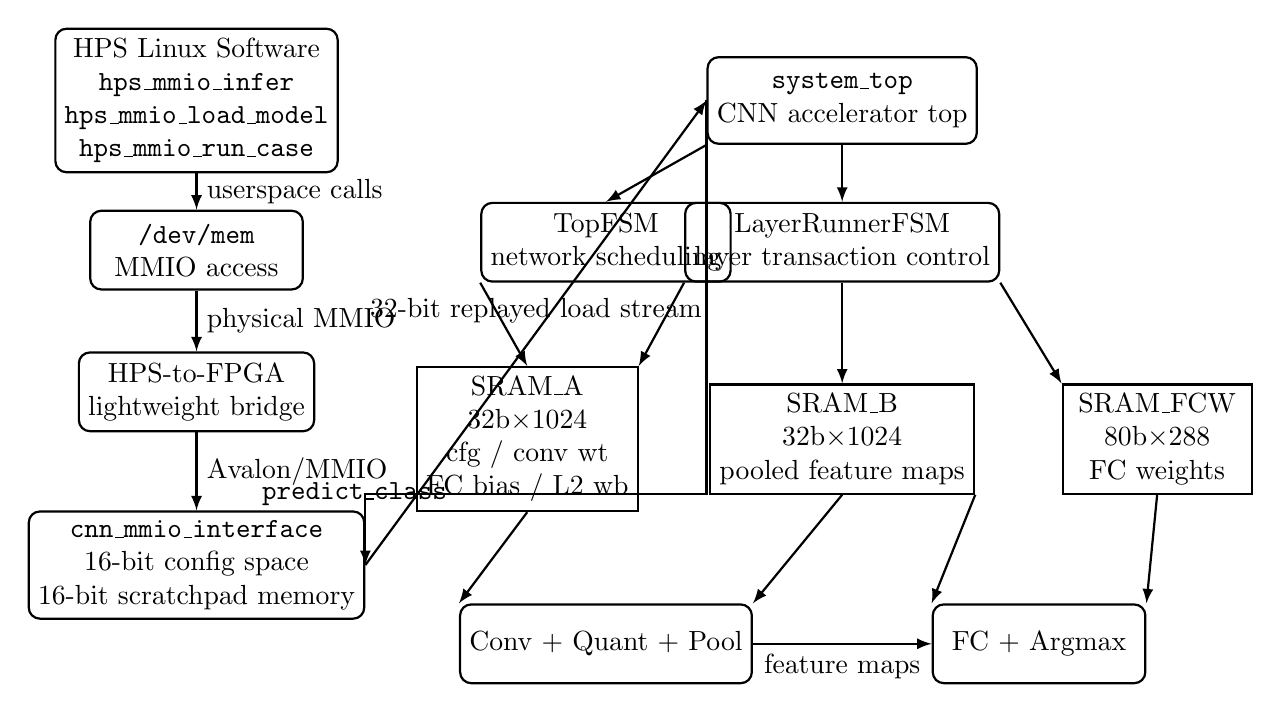
\begin{tikzpicture}[
    x=1cm, y=1cm,
    block/.style={draw, thick, rectangle, rounded corners, align=center, minimum width=3.2cm, minimum height=1.1cm},
    smallblock/.style={draw, thick, rectangle, rounded corners, align=center, minimum width=2.7cm, minimum height=1cm},
    memblock/.style={draw, thick, rectangle, align=center, minimum width=2.4cm, minimum height=1.2cm},
    line/.style={draw, thick, -latex}
]

\node[block] (hpssw) at (0,8.5) {HPS Linux Software\\\texttt{hps\_mmio\_infer}\\\texttt{hps\_mmio\_load\_model}\\\texttt{hps\_mmio\_run\_case}};
\node[smallblock] (devmem) at (0,6.6) {\texttt{/dev/mem}\\MMIO access};
\node[smallblock] (bridge) at (0,4.8) {HPS-to-FPGA\\lightweight bridge};
\node[block] (mmio) at (0,2.6) {\texttt{cnn\_mmio\_interface}\\16-bit config space\\16-bit scratchpad memory};

\node[block] (sys) at (8.2,8.5) {\texttt{system\_top}\\CNN accelerator top};
\node[smallblock] (topfsm) at (5.2,6.7) {TopFSM\\network scheduling};
\node[smallblock] (runner) at (8.2,6.7) {LayerRunnerFSM\\layer transaction control};

\node[memblock] (srama) at (4.2,4.2) {SRAM\_A\\32b$\times$1024\\cfg / conv wt\\FC bias / L2 wb};
\node[memblock] (sramb) at (8.2,4.2) {SRAM\_B\\32b$\times$1024\\pooled feature maps};
\node[memblock] (sramfcw) at (12.2,4.2) {SRAM\_FCW\\80b$\times$288\\FC weights};

\node[smallblock] (conv) at (5.2,1.6) {Conv + Quant + Pool};
\node[smallblock] (fc) at (10.7,1.6) {FC + Argmax};

\draw[line] (hpssw) -- node[right] {userspace calls} (devmem);
\draw[line] (devmem) -- node[right] {physical MMIO} (bridge);
\draw[line] (bridge) -- node[right] {Avalon/MMIO} (mmio);
\draw[line] (mmio.east) -- node[above] {32-bit replayed load stream} (sys.west);

\draw[line] (sys.south west) -- (topfsm.north);
\draw[line] (sys.south) -- (runner.north);

\draw[line] (topfsm.south west) -- (srama.north);
\draw[line] (runner.south west) -- (srama.north east);
\draw[line] (runner.south) -- (sramb.north);
\draw[line] (runner.south east) -- (sramfcw.north west);

\draw[line] (srama.south) -- (conv.north west);
\draw[line] (sramb.south) -- (conv.north east);
\draw[line] (sramb.south east) -- (fc.north west);
\draw[line] (sramfcw.south) -- (fc.north east);

\draw[line] (conv.east) -- node[below] {feature maps} (fc.west);
\draw[line] (sys.west) |- ++(-2.0,-5.0) -| node[pos=0.25,left] {\texttt{predict\_class}} (mmio.east);

\end{tikzpicture}
\caption{System block diagram of the CNN accelerator project.}
\label{fig:system-block-diagram}
\end{figure}

The main responsibilities of each block are:
\begin{itemize}
\item The HPS software loads preload files, writes scratchpad contents, starts
transactions, and polls for completion.
\item The HPS-to-FPGA lightweight bridge transports MMIO accesses from the ARM
cores into the FPGA fabric.
\item \texttt{cnn\_mmio\_interface} exposes a 16-bit register space and a
16-bit scratchpad memory, then reconstructs the original 32-bit load words
needed by the CNN datapath.
\item \texttt{TopFSM} controls high-level model load and inference sequencing.
\item \texttt{LayerRunnerFSM} manages per-layer execution and SRAM accesses.
\item \texttt{SRAM\_A}, \texttt{SRAM\_B}, and \texttt{SRAM\_FCW} hold
configuration words, weights, intermediate feature maps, and FC weights.
\item The datapath consists of a convolution/quantization/pooling pipeline
followed by a final fully-connected stage and argmax classifier.
\end{itemize}

\section{Algorithms}

The accelerator implements a fixed CNN inference pipeline. The model parameters
are precomputed offline and stored as preload files. During execution, the
system performs three main steps:
\begin{enumerate}
\item load network configuration and weights into the accelerator memory system
\item stream a single input image through the convolutional pipeline
\item run the fully-connected layer and output the predicted class
\end{enumerate}

The convolutional portion of the datapath performs layer-by-layer processing
with quantization and pooling between stages. Intermediate feature maps are
stored in SRAM and reused by later stages. The final fully-connected stage
computes the class logits and an argmax operation selects the predicted digit or
gesture class.

The current host-side flow uses two distinct software-triggered transactions:
\begin{itemize}
\item \textbf{Model load}: replay convolution configuration, convolution
weights, FC bias, and FC weights into the accelerator
\item \textbf{Inference}: replay the input image and wait for the prediction
result
\end{itemize}

\section{The Hardware/Software Interface}

The CNN accelerator is exposed to the HPS as a 16-bit memory-mapped peripheral.
The HPS software stages model parameters and input data in a scratchpad memory,
programs the control registers, and polls the status registers until execution
completes. The MMIO wrapper then replays the staged data into the original
\texttt{system\_top} streaming datapath.

The interface uses two address regions:
\begin{itemize}
\item \textbf{Memory space} (\texttt{address[19] = 0}): 16-bit scratchpad storage
\item \textbf{Configuration space} (\texttt{address[19] = 1}): 16-bit control and status registers
\end{itemize}

\subsection{Register Map}

All registers are 16 bits wide. Table~\ref{tab:mmio-reg-map} summarizes the
register interface exposed by the MMIO wrapper.

\begin{table}[h]
\centering
\small
\begin{tabular}{|l|c|c|p{7.2cm}|}
\hline
\textbf{Register} & \textbf{Index} & \textbf{Access} & \textbf{Description} \\
\hline
\texttt{CONTROL} & 0 & WO & start model load, start inference, clear status \\
\hline
\texttt{STATUS} & 1 & RO & busy flag, model-loaded flag, done flag, predicted class \\
\hline
\texttt{CONV\_CFG\_BASE} & 2 & RW & base halfword address of convolution configuration segment \\
\hline
\texttt{CONV\_CFG\_LEN} & 3 & RW & number of 32-bit words in convolution configuration segment \\
\hline
\texttt{CONV\_WT\_BASE} & 4 & RW & base halfword address of convolution weight segment \\
\hline
\texttt{CONV\_WT\_LEN} & 5 & RW & number of 32-bit words in convolution weight segment \\
\hline
\texttt{FC\_BIAS\_BASE} & 6 & RW & base halfword address of FC bias segment \\
\hline
\texttt{FC\_BIAS\_LEN} & 7 & RW & number of 32-bit words in FC bias segment \\
\hline
\texttt{FCW\_BASE} & 8 & RW & base halfword address of FC weight segment \\
\hline
\texttt{FCW\_LEN} & 9 & RW & number of 32-bit words in FC weight segment \\
\hline
\texttt{IMAGE\_BASE} & 10 & RW & base halfword address of input image segment \\
\hline
\texttt{IMAGE\_LEN} & 11 & RW & number of 32-bit words in input image segment \\
\hline
\texttt{PREDICT} & 12 & RO & latched predicted class \\
\hline
\texttt{IF\_ERROR} & 13 & RO & interface error flags \\
\hline
\end{tabular}
\caption{MMIO register map.}
\label{tab:mmio-reg-map}
\end{table}

\subsection{Register Fields}

Table~\ref{tab:mmio-fields} lists the meaning of each implemented control and
status bit.

\begin{table}[h]
\centering
\small
\begin{tabular}{|l|l|p{8.1cm}|}
\hline
\textbf{Register} & \textbf{Bits} & \textbf{Meaning} \\
\hline
\texttt{CONTROL} & bit 0 & start model preload replay \\
\hline
\texttt{CONTROL} & bit 1 & start inference replay \\
\hline
\texttt{CONTROL} & bit 2 & clear \texttt{predict\_done} and \texttt{IF\_ERROR} \\
\hline
\texttt{CONTROL} & bits 15:3 & reserved, write zero \\
\hline
\texttt{STATUS} & bit 0 & reserved \\
\hline
\texttt{STATUS} & bit 1 & replay engine busy \\
\hline
\texttt{STATUS} & bit 2 & model preload complete \\
\hline
\texttt{STATUS} & bit 3 & inference complete \\
\hline
\texttt{STATUS} & bits 7:4 & predicted class \\
\hline
\texttt{STATUS} & bits 15:8 & reserved \\
\hline
\texttt{PREDICT} & bits 3:0 & predicted class \\
\hline
\texttt{PREDICT} & bits 15:4 & reserved \\
\hline
\texttt{IF\_ERROR} & bit 0 & model load requested while busy \\
\hline
\texttt{IF\_ERROR} & bit 1 & inference requested while busy \\
\hline
\texttt{IF\_ERROR} & bit 2 & inference requested before model load completed \\
\hline
\texttt{IF\_ERROR} & bit 3 & low halfword scratchpad read out of range \\
\hline
\texttt{IF\_ERROR} & bit 4 & high halfword scratchpad read out of range \\
\hline
\texttt{IF\_ERROR} & bits 15:5 & reserved \\
\hline
\end{tabular}
\caption{Implemented control and status bit definitions.}
\label{tab:mmio-fields}
\end{table}

\subsection{Scratchpad Address Map}

The software stores all staged data in the scratchpad memory before writing the
\texttt{CONTROL} register. The scratchpad is 16-bit addressed, so each logical
32-bit word occupies two consecutive halfword locations. The default layout is
shown in Table~\ref{tab:mmio-scratchpad}.

\begin{table}[h]
\centering
\small
\begin{tabular}{|l|c|c|l|}
\hline
\textbf{Segment} & \textbf{Base (halfwords)} & \textbf{Length (32-bit words)} & \textbf{Content} \\
\hline
\texttt{conv\_cfg} & 0 & 45 & convolution configuration \\
\hline
\texttt{conv\_wt} & 90 & 225 & convolution weights \\
\hline
\texttt{fc\_bias} & 540 & 10 & fully-connected bias \\
\hline
\texttt{fcw} & 560 & 864 & fully-connected weights \\
\hline
\texttt{image} & 2288 & 1024 & input image \\
\hline
\end{tabular}
\caption{Default scratchpad layout.}
\label{tab:mmio-scratchpad}
\end{table}

\begin{figure}[h]
\centering
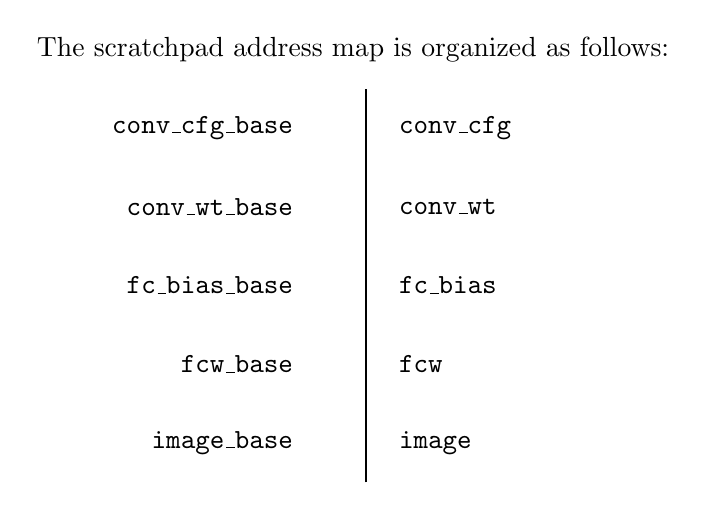
\begin{tikzpicture}[x=1cm,y=1cm]
\node[anchor=west] at (0,5.8) {The scratchpad address map is organized as follows:};

\node[anchor=east] at (3.5,4.8) {\texttt{conv\_cfg\_base}};
\node[anchor=east] at (3.5,3.8) {\texttt{conv\_wt\_base}};
\node[anchor=east] at (3.5,2.8) {\texttt{fc\_bias\_base}};
\node[anchor=east] at (3.5,1.8) {\texttt{fcw\_base}};
\node[anchor=east] at (3.5,0.8) {\texttt{image\_base}};

\draw[thick] (4.3,0.3) -- (4.3,5.3);

\node[anchor=west] at (4.6,4.8) {\texttt{conv\_cfg}};
\node[anchor=west] at (4.6,3.8) {\texttt{conv\_wt}};
\node[anchor=west] at (4.6,2.8) {\texttt{fc\_bias}};
\node[anchor=west] at (4.6,1.8) {\texttt{fcw}};
\node[anchor=west] at (4.6,0.8) {\texttt{image}};
\end{tikzpicture}
\caption{Scratchpad memory organization.}
\label{fig:mmio-address-layout}
\end{figure}

\subsection{Transaction Sequence}

Each logical 32-bit word is written into the scratchpad as two consecutive
16-bit halfwords. The MMIO wrapper reconstructs the original 32-bit word before
forwarding it to the accelerator input stream.

One inference transaction proceeds as follows:
\begin{enumerate}
\item Write preload data and input image into the scratchpad memory.
\item Program the base and length registers.
\item Write \texttt{CONTROL[0]} to start model loading.
\item Poll \texttt{STATUS[2]} until model loading completes.
\item Write \texttt{CONTROL[1]} to start inference.
\item Poll \texttt{STATUS[3]} until inference completes.
\item Read \texttt{PREDICT} and \texttt{IF\_ERROR}.
\end{enumerate}


\section{Resource Budgets}

The accelerator is targeted to the Cyclone V device on the DE1-SoC board
(\texttt{5CSEMA5F31C6}). The current design fits functionally in simulation and
supports HPS-side MMIO control, but timing closure remains the primary hardware
risk for final board deployment.

The implementation makes heavy use of SRAM-backed storage and arithmetic
resources in the convolution and fully-connected stages. The most timing- and
resource-sensitive blocks are:
\begin{itemize}
\item the convolution datapath and its accumulation pipeline
\item the FC stage and packed FC weight access path
\item the control-to-memory fanout around the layer runner and SRAM wrappers
\item the MMIO wrapper replay engine, which must preserve the original
streaming contract of \texttt{system\_top}
\end{itemize}

At the current stage of the project, functional correctness has been established
through behavioral simulation and MMIO smoke testing, while full DE1-SoC system
integration remains limited by Platform Designer custom-IP packaging and
slow-corner timing closure.

\end{document}
